\documentclass[11pt,a4paper]{article}

\usepackage[margin=1in, paperwidth=8.3in, paperheight=11.7in]{geometry}
\usepackage{amsmath,amsfonts,fancyhdr,bbm,graphicx,tikz,float}
\usetikzlibrary{automata,positioning}
\graphicspath{ {img/} }
\usepackage[section,nohyphen]{DomH}
\headertitle{Financial Mathematics - Notes}

\begin{document}

\title{Financial Mathematics - Notes}
\author{Dom Hutchinson}
\date{\today}
\maketitle

\tableofcontents\newpage

\section{Financial Terminology \& Single-Period Models}\label{sec_financial_terminology_and_single_period_model}

  \begin{proposition}{Types of Financial Objects}
    In this course we consider two types of financial objects
    \begin{enumerate}
      \item \textit{Underlying Traded Assets} (e.g. Oil, interest rates \& exchange rates).
      \item \textit{Derivative Securities} (contracts based on \textit{Underlying Traded Assets})
    \end{enumerate}
  \end{proposition}

  \begin{proposition}{Derivative Securities}
    \textit{Derivative Securities} can act as insurance, by paying the holder when the value of the \textit{Underlying Traded Asset} goes in the opposite direction.
    \par \textit{e.g.} ``I will pay you £1mn for every dollar the price of oil is over £80 on 1st December 2025.''
    \par Our question is what such a contract is worth. To answer this we consider both \textit{Arbitrage} and \textit{Modelling}.
  \end{proposition}

  \begin{definition}{Modelling}
    \textit{Modelling} is the practice of forecasting the future value of an \textit{Underlying Traded Asset}. Classical models for price processes involve \textit{Brownian Motion}.
  \end{definition}

  \begin{definition}{Arbitrage}\label{def_arbitrage}
    \textit{Arbitrage} is the possibility of being able to make a profit on a transaction without being exposed to the risk of incurring a loss. Traders who try to lock in riskless profit are called \textit{Arbitrageurs}.
    \par Generally realised by buying and selling the same asset in different markets, with the asset having a different value in each market.
    \par (\arabic{definition})
  \end{definition}

  \begin{example}{Arbitrage}
    Consider a stock that is traded on both the NYSE and the LSE. Suppose the sotck price is \$189 on the NYSE and £100 on the LSE, and the exchange rate is \$1.87=£1. The following \textit{Arbitrage Opportunity} exists:
    \begin{enumerate}
      \item Buy 100 shares in London.
      \item Sell all these shares in NY.
      \item Exchange dollars to sterling.
    \end{enumerate}
    This has a riskless profit of \$200=£106.95 (assuming negligible transaction costs).
  \end{example}

  \begin{proposition}{"No Arbitrage Principle"}
    The \textit{"No Arbitrage Principle"} is the principle that \textit{Arbitrage} opportunity do not exist (for long) in real life markets. If they did then the market activity caused by agents exploiting the \textit{Arbitrage} opportunity\footnote{The forces of \textit{Supply-and-Demand}.} would raise the cost of buying and thus remove the \textit{Arbitrage} opportunity.
  \end{proposition}

  \begin{remark}{Arbitrage \& Valuing Contracts}
    When valuing contracts we assume there is no arbitrage (The \textit{"No Arbitrage Principle"}). This means we can decide a single price for a contract, as at any other price there would be arbitrage.
  \end{remark}

  \begin{definition}{Short Selling}
    \textit{Short Selling} is the practice of borrowing an asset, selling it and then at some point in the future buying an equivalent asset to reimburse whoever lent you the original asset. If the value of the asset has fallen in this time then you make a profit.
  \end{definition}

  \begin{example}{}
    Consider a share which trades at £10 on 1st Jan. Suppose we know that on 1st July there is a 2/3 chance it will be worth £25 and 1/3 chance it will be worth £5. Suppose the following contract is offer on the 1st Jan:
    \begin{enumerate}
      \item ``If the share goes up, I will pay you £4. If the share price goes down, I pay you nothing.''
    \end{enumerate}
    What is this contract worth? (Assuming your bank account pays no interest).
    \par You could argue that the contract should be worth the expected payout of the contract , $\frac23\times\pounds4+\frac13\times\pounds0=\pounds2.66$.
    \par However, consider creating a replicating portfolio which buys $\frac15$ of a unit of the stock and borrows £1 from the bank. On 1st Jan this portfolio is worth $(1/5)\times\pounds10-\pounds1=\pounds1$.
    \begin{itemize}
      \item If the stock goes up, the portfolio is worth $\frac15\times\pounds25-\pounds1=\pounds4$.
      \item If the stock goes down, the portfolio is worth $\frac15\times\pounds5-\pounds1=\pounds0$.
    \end{itemize}
    These two outcomes show that this replicating portfolio has exactly the same payouts as the contract being offer. This means that whatever the portfolio costs, the contract must cost the same.
    \par Suppose the portfolio costs £1 and the contract costs £1.50. Then you would sell the contract, buy the portfolio and make £0.50 profit independent of the price of the share on 1st July. (and visa-versa).
    \par This valuation is independent of the probability of the asset's value increasing, but there is an interesting ``phantom probability'' $q=\frac14$. The price of the contract is the expected payout of the contract, if the probability of the share price increasing was $q$, $\expect[\text{payout}]=\frac14\times\pounds4+\frac34\times0=\pounds1$. Also, using this probability the expected value of the stock on July 1st is $\frac14\times\pounds25+\frac34\times\pounds5=\pounds10$, the same as it was on Jan 1st. (This is how we find $q$).
    \par This $q$ is known as the \textit{Equivalent Martingale Measure}
  \end{example}

  \begin{definition}{Equivalent Martingale Measure}
    TODO
  \end{definition}

  \begin{remark}{Value of Money}
    These problems are more interesting when we consider that the value of money is not constant due to inflation \& interest rates.
  \end{remark}

  \begin{remark}{Risk-Free}
    When referring to an activity being ``Risk-Free'' we mean that the loses \& profits from it are known, not that there are no loses.
  \end{remark}

  \begin{definition}{Bank Process, $B_t$}
    \textit{Bank Process}, $B_t$, is a measure of how much the value of money has changed over $t$ time-periods.
    \par Assume the existence of a risk-free bank account with known interest rate $r$ (assumed to be constant over interval $[0,T]$). This means the initial deposit of one unit becomes the following after $t$ time-steps
    \begin{itemize}
      \item[Continuous Time Model] $B_t=e^{rt}$
      \item[Multi-Period Model] $B_t=(1+r)^t$
    \end{itemize}
    We must consider the performance of our portfolio relative to the \textit{Bank Process}, by discounting our profits by factor $B_t$.
    \par \textit{N.B.} - The \textit{Bank Process} is also known as a \textit{Bond} or a \textit{Numeraire}.
  \end{definition}

  \begin{definition}{Derivative Security}
    A \textit{Derivative Security} is a contract whose value at expiration date $T$ is a function of the values of the assets within the time interval $[0,T]$. Often, the value is just a function of the value at time $T$.
  \end{definition}

  \begin{definition}{Forward Contract}
    A \textit{Forward Contract} is an agreement to buy or sell an asset $S$ at future \textit{Delivery Date}\footnote{AKA \textit{Settlement Date}} $T$ for \textit{Delivery Price} $K$. Both parties are obliged to fulfil the contract.
    \par The agent who agrees to buy the underlying asset is said to have a \textit{Long Position}, the other agent has a \textit{Short Position}.
    \par The \textit{Forward Price} $f(t;T)$ is the delivery price which would make the contract have zero value at time $t$.
  \end{definition}

  \begin{remark}{Usefulness of Forward Contracts}
    \textit{Forward Contracts} allow you to agree terms of a future purchase/sale in advance of actually transacting. This means you know the price you will receive/pay and thus can plan accordingly. (e.g. Farmers may agree to price per tonne of corn well before the harvest).
  \end{remark}

  \begin{definition}{Option Contract}
    An \textit{Option} is a financial instrument giving one the right, but \underline{not} the obligation, to buy or sell an asset $S$ at (or before) a specified date $T$ for an agreed \textit{Strike Price}\footnote{AKA \textit{Exercise Price}} $K$. There are two classes of \textit{Option Contract}
    \begin{itemize}
      \item \textit{Call Option} - The holder has the right to buy.
      \item \textit{Put Option} - The holder has the right to sell
    \end{itemize}
    \textit{N.B.} Only one party (the holder) decides whether to exercise the contract or not, the other (the writer) has to do what the former wishes.
  \end{definition}

  \begin{definition}{European \& American Options}
    \textit{European} vs \textit{American Options} determine when the \textit{Option Contract} can be exercised.
    \begin{itemize}
      \item \textit{European Option} can only be executed on the expiry date.
      \item \textit{American Option} can be executed on any date up to and inc. the expiry date.
    \end{itemize}
  \end{definition}

  \begin{example}{Derivative}
    Consider the following call option
    \begin{quote}
      ``The holder has the right to buy 1,000 litres of petrol for £1,000 next Jan 1st''
    \end{quote}
    If the market price $S_T$ on 1st Jan is greater than £1,000 it is profitable to exercise the option. You would make profit $S_T-1000$. However, if $S_T$ was less than £1,000 then it is better to buy petrol at the market price.
    \par The value on Jan 1st of the option will be $\{S_T-1000\}_+$, a function of the random price $S_T$.
    \par \textit{N.B.} - a put option would the opposite analysis with profit $1000-S_T$.
  \end{example}

  \begin{definition}{Dividend}
    A \textit{Dividend} is a one-off payment provided made to the holder of an underlying asset at a certain time. Not all underlying assets provide a \textit{Dividend}.
  \end{definition}

  \begin{proposition}{Fair Price of a Forward Contract with a Dividend}\label{prop_fair_price_of_forward_w_dividend}
    Consider a forward contract on an asset with current price $S_0$ which provides a known dividend $D$ at time point $t_0\in(0,T)$ and has delivery date $T$.
    \par Assume the existence of a risk-free bank account with constant interest rate $r$ during the interval $[0,T]$. This means an initial deposit of one unit grows to $B_t=e^{rt}$ up to time point $t$.
    \par If $D=0$ (ie no dividend is paid) then the fair delivery price for the forward contract is $K=S_0e^{rT}$. Else, if $D>0$ (ie a dividend is paid) then the fair delivery price for the forward contract is $K=(S_0-I)e^{rT}$ where $I=De^{-rt_0}$.
  \end{proposition}

  \begin{proof}{Proposition \ref{sec_financial_terminology_and_single_period_model}.\ref{prop_fair_price_of_forward_w_dividend}}
    We use the ``no-arbitrage principle'' to prove that this is the fair price.
    \par First assume that the price of the contract is $K>(S_0-I)e^{rT}$ where $I=De^{-rt_0}$. Then an arbitrageur will adopt a short position on this contract by doing the following
    \begin{enumerate}
      \item Borrow $\pounds£S_0$ at an interest rate of $r$.
      \item Buy the underlying asset.
      \item Take a short position in the forward contract (i.e. agree to sell the asset for $K$ at time $T$).
    \end{enumerate}
    At time point $T_0$ we use the dividend to partially repay the loan. Finally, at time point $T$ we sell the asset for $K$ and repay the outstanding balance of the loan. The riskless profit is $K-(S_0e^{rt_0}D)e^{(T-t_0)}=K-(S_0-I)e^{rT}$, regardless of the price of the underlying asset at time point $T$.
    \par Now assume the converse, the price of the contract is $K-(S_0-I)e^{rT}>0$ where $I=De^{-rt_0}$. Then an arbitrageur will adopt a long position on this contract by doing the following
    \begin{enumerate}
      \item Short sell the underlying asset (N.B. you are obliged to pay dividends to the lender).
      \item Invest the proceeds of $S_0$ at the risk-free interest rate of $r$.
      \item Take a long position in the forward contract (i.e. agree to buy the asset for $K$ at time $T$).
    \end{enumerate}
    At time $t_0$ we have to pay the dividend from our bank account. On the delivery date the arbitrageur buys the asset for $K$ and makes a riskless profit of $(S_0e^{rt_0}-D)e^{r(T-t_0)}-K=(S_0-I)e^{rT}-K>0$ where $I=De^{-rt_0}$.\footnote{$D$ is subtracted as you have to pay the lender the dividend, but as you have already sold the asset you do not receive the dividend from the asset.}
  \end{proof}

  \begin{theorem}{Equivalent Contract Valuations over Time}\label{thrm_equivalent_contract_valuations_over_time}
    Consider two combinations of financial derivatives that both have the same value $V=W$ at time point $T$. Then their prices $V_t$ and $W_t$ at time point $t<T$ must also coincide.
  \end{theorem}

  \begin{proof}{Theorem \ref{sec_financial_terminology_and_single_period_model}.\ref{thrm_equivalent_contract_valuations_over_time}}
    We use the ``no-arbitrage principle'' and assume WLOG that $V_t>W_t$. Then, at time $t$, we would do the following
    \begin{enumerate}
      \item Sell or short the first combination.
      \item Buy the second combination.
      \item Invest the difference $V_t-W_t>0$.
    \end{enumerate}
    At time point $T$ we would do the following
    \begin{enumerate}
      \item Buy the second combination for $W$.
      \item Sell the first combination for $V=W$.
    \end{enumerate}
    The risk-free profit, assuming a risk-free interest rate of $r$, is $(V_t-W_t)e^{r(T-t)}>0$
  \end{proof}

  \begin{proposition}{Put-Call Parity}
    We apply \texttt{Theorem \ref{sec_financial_terminology_and_single_period_model}.\ref{thrm_equivalent_contract_valuations_over_time}} to \textit{European Put \& Call Options}.
    \par Consider a \textit{European Put Option} and a \textit{European Call Option} for the same underlying asset, both with strike price $K$ and expiry date $T$. Assume that $S_T$ is the price of the underlying asset at time point $T$ then the payoff of the \textit{Call Option} is $C$ and the \textit{Put Option} is $P$ at time $T$, where
    \[\begin{array}{rcl}
      C&=&\{S_T-K\}_+\\
      P&=&\{K-S_T\}_+
    \end{array}\]
    For the first combination choose the \textit{Underlying Asset} and \textit{European Put Option}. The value of this combination at time point $T$ is $V=S_T+P=\max\{S_T,K\}$.
    \par For the second combination choose the \textit{European Call Option} and a bond which matures at time point $T$ with a price of $K$. The value of the second combination is $W=K+C=\max\{S_T,K\}$
  \end{proposition}

  \begin{theorem}{Put-Call Parity - Formal}
    Let $S_t$ be the price of the asset at time point $t$, $Ke^{-r(T-t)}$ the discounted value of the bond and $C_t,P_t$ be the prices of the \textit{European Call} and \textit{Put Options} at time $t$, respectively. Then
    \[ S_t+P_t-C_t=Ke^{-r(T-t)}\quad\ \forall t\in[0,T] \]
    If, at some time $t$, this relationship does not hold then an \textit{Arbitrage Opportunity} exists at this time.
  \end{theorem}

  \begin{theorem}{Lower Bound for a European Call Option}
    We can use \textit{Put-Call Parity} to determine a lower bound for a \textit{European Call Option}
    \[\begin{array}{rcl}
      S_t+P_t-C_t&=&Ke^{-r(T-t)}\\
      \implies C_t&=&S_t+P_t-Ke^{-r(T-t)}\\
      \implies C_t\geq\{S_t-Ke^{-r(T-t)}\}_+\text{ as }P_t\geq0
    \end{array}\]
  \end{theorem}

  \begin{theorem}{American Call Options}\label{thrm_american_call_option_value}
    Let $C_A$ be the price of an \textit{American Call Option} and $C_E$ be the price of a \textit{European Call Option} for the same underlying asset, with the same strike price and expiry date.
    \par Then, for a \underline{non-dividend paying} stock we have that
    \[ C_A=C_E \]
    This means that, for non-dividend paying stock, it is suboptimal to exercise an American call optional early.
  \end{theorem}

  \begin{proof}{Theorem \ref{sec_financial_terminology_and_single_period_model}.\ref{thrm_american_call_option_value}}
    First, note that exercising the American call early at time $t<T$ generates an income of $S_t-K$. However, from the inequality above, we know that selling the call options yields a cash-flow of $\{S_t-Ke^{-r(T-t)}\}_+\geq S_t-Ke^{-r(T-t)}$. Since $e^{-r(T-t)}<1$, exercising the call at any $t<T$ (i.e. early) is suboptimal.
  \end{proof}

\subsection{Single-Period Model}

  \begin{definition}{Sample Space, $\Omega$}
    The \textit{Sample Space} $\Omega$ is the set consisting of all elementary outcomes.
  \end{definition}

  \begin{definition}{Random Variable}
    A \textit{Random Variable} $X$ is a function from the \textit{Sample Space} to real numbers
    \[ X:\Omega\to\reals \]
  \end{definition}

  \begin{definition}{Single-Period Model}
    The \textit{Single-Period Model} is a model for a financial market with the following components
    \begin{itemize}
      \item Initial date $t=0$ and terminal date $t=1$, with trading and consumption only allowed on these two dates.
      \item A finite \textit{Sample Space} $\Omega$ with $|\Omega|=K<\infty$.
      \[ \Omega=\{\omega_1,\dots,\omega_k\} \]
      with each element corresponding to some state of the world.
      \item A \textit{Probability Measure} $\prob$ on $\Omega$ with $\prob(\omega_i)>0\ \forall\ \omega_i\in\Omega$.
    \end{itemize}
  \end{definition}

  \begin{definition}{Bank Account Process $B$}
    A \textit{Bank Account Process} $B=\{B_t:t=0,1\}$ where $B_0=1$ and $B_1$ is a \textit{Random Variable}.
    \par The \textit{Bank Account Process} is distinguished from other securities because its price $B_1(\omega)$ at time $t=1$ is assumed to be strictly positive for all $\omega\in \Omega$. Usually, in fact, $B_1\geq1$ in which case $B_1$ should be though of as the value of the bank account at time $t=1$, if 1 unit of currency was deposited at time $t=0$. And, $r=B_t-1\geq0$ should be thought of as the \textit{Interest Rate}. In many applications $r$ and $B_1$ are deterministic scalars.
  \end{definition}

  \begin{definition}{Price Process\footnote{AKA \textit{Stock Process}}}
    A \textit{Price Process} $S=\{S(t):t=0,1\}$ where $S(t)=(S_1(t),S_2(t),\dots,S_N(t)),\ N<\infty$ and $S_i(t)$ is the price of the $i^{th}$ security at time $t$. In many applications these $N$ risky securities are stocks.
    \par The prices at time $t=0$ are positive scalars that are known to the investors, whereas the prices at time $t=1$ are non-negative random variables whose value only become known to investors at time $t=1$.
  \end{definition}

  \begin{definition}{Trading Strategy $H$}
    A \textit{Trading Strategy} $H=(H_0,\dots,H_N)$ describes an investor's portfolio as carried from time $t=0$ to time $t=1$. Specifically, $H_0$ is the number of units of the currency invested in the \textit{Savings Account} and $H_i$ with $i\geq1$ is a scalar of the number of units invested in the $i^{th}$ security.
    \par Note that $H_i$ can be positive or negative. Positive means you have bought/invested and negative means you are borrowing or short selling.
  \end{definition}

  \begin{example}{Single-Period Model (Zero Interest)}
    Consider a share which trades on 1st Jan for £10. Suppose we know with probability $p_1=\frac23$ it will be worth £25 on 1st July, and with probability $p_2=\frac13$ it will be worth £5 on 1st July. You also have access to a bank account which pays no interest ($r=0$), which you can pay into or borrow from. Create a \textit{Replicating Portfolio} as follows: buy $\frac15$ unit of the stock, and borrow £1 from the bank.
    \par We can rephrase this as a \textit{Single-Period Model} for a single period ($T=1$).
    \begin{itemize}
      \item \textit{Bank Account Process} - $B_0=B_1=1$. As no interest rate.
      \item \textit{Sample Space} - $\Omega=\{\omega_1,\omega_2\}$ with $\omega_1$ being the event the stock rises to £25 and $\omega_2$ being the event the stock falls to £5.
      \item There are $N=1$ stocks. So the \textit{Price Process} is
      \[\begin{array}{rcl}
        S_1(0)(\omega_i)&=&10\text{ for }i=1,2\\
        S_1(1)(\omega_i)&=&\begin{cases}
          25&\text{if }i=1\\
          5&\text{if }i=2
        \end{cases}
      \end{array}\]
      \item We can write the \textit{Replicating Portfolio} as a vector $(H_0,H_1)$.
    \end{itemize}
  \end{example}

  \begin{definition}{Value Process, $V$}
    A \textit{Value Process} $V=\{V_t:t=0,1\}$ describes the total value of the portfolio at each point in time
    \[ V_t=H_0B_t+\sum_{n=1}^NH_nS_n(t) \]
  \end{definition}

  \begin{definition}{Gains Process, $G$}
    The \textit{Gains Process} $G$ is a random variable that describes the total profit or loss generated by the portfolio between times 0 and 1.
    \[ G=H_0r+\sum_{n=1}^NH_n\Delta S_n \]
    where $\Delta S_n=S_n(1)-S_n(0)$ is the change in price of the $n^{th}$ asset.
  \end{definition}

  \begin{remark}{Normalising Prices}
    It is convenient to normalize the prices, so that the bank account becomes constant by defining discounted versions of the processes defined earlier. See \texttt{Definitions \ref{sec_financial_terminology_and_single_period_model}.\ref{def_discounted_price_process}, \ref{sec_financial_terminology_and_single_period_model}.\ref{def_discounted_value_process}, \ref{sec_financial_terminology_and_single_period_model}.\ref{def_discounted_gains_process}}.
  \end{remark}

  \begin{definition}{Discounted Price Process, $S^*$}\label{def_discounted_price_process}
    A \textit{Discounted Price Process} $S^*$ is the \textit{Price Process} $S$ normalised by the \textit{Bank Process} $B_t$
    \[S^*:=\{S_t^*:t=0,1\}\text{ with }S_n^*(t):=\frac{S_n(t)}{B_t}\text{ for }n\in\{1,\dots,N\},\ t=\{0,1\}\]
  \end{definition}

  \begin{definition}{Discounted Value Process, $V^*$}\label{def_discounted_value_process}
    A \textit{Discounted Value Process} $V_t^*$ is the \textit{Value Process} $V_t$ normalised by the \textit{Bank Process} $B_t$
    \[ V_t^*:=\frac{V_t}{B_t}=H_0+\sum_{n=1}^NH_nS_n^*(t)\text{ for }t=0,1 \]
  \end{definition}

  \begin{definition}{Discounted Gains Process, $G^*$}\label{def_discounted_gains_process}
    A \textit{Discounted Gains Process} $G^*$is the \textit{Gains Process} $G$ normalised by the \textit{Bank Process} $B_t$
    \[ G^*:=\frac{G}{B_t}=\sum_{n=1}^NH_n\Delta S_n^*\text{ with }\Delta S_n^*:=S_n^*(1)-S_n^*(0) \]
  \end{definition}

  \begin{example}{Single-Period Model (Non-Zero Interest)}
    Consider a share which trades on 1st Jan for £10. Suppose we know with probability $p_1=\frac23$ it will be worth £25 on 1st July, and with probability $p_2=\frac13$ it will be worth £5 on 1st July. You also have access to a bank account which pays interest $r\in\reals$, which you can pay into or borrow from.
    \par We can rephrase this as a \textit{Single-Period Model} for a single period ($T=1$).
    \begin{itemize}
      \item Bank Account Process - $B_0=1,\ B_1=1+r$.
      \item Probability Space - $\Omega=\{\omega_1,\omega_2\}$ where $\omega_1$ indicates the stock going up and $\omega_2$ indicates the stock going down.
      \item There is $N=1$ units of the stock, so we have the following price process
      \[\begin{array}{rcl}
        S_1(0)(\omega_i)&=&10\text{ for }i\in\{1,2\}\\
        S_1(1)(\omega_1)&=&25\\
        S_1(1)(\omega_2)&=&5
      \end{array}\]
      And discounted price process
      \[\begin{array}{rcl}
        S^*_1(0)(\omega_i)&=&10\text{ for }i\in\{1,2\}\\
        S^*_1(1)(\omega_1)&=&\frac{25}{1+r}\\
        S^*_1(1)(\omega_2)&=&\frac5{1+r}
      \end{array}\]
      \item For an arbitrary strategy $H$, our portfolio has initial value $V_0=V_0^*=H_0+10H_1$. Thus, we can determine the gains and future values of this portfolio
      \[\begin{array}{rcl}
        V_1(\omega_1)&=&(1+r)H_0+25H_1\\
        V_1^*(\omega_1)&=&H_0+\frac{25}{1+r}H_1\\
        G(\omega_1)&=&rH_0+15H_1\\
        G^*(\omega_1)&=&\left(\frac{25}{1+r}-10\right)H_1\\
        V_1(\omega_2)&=&(1+r)H_0+5H_1\\
        V_1^*(\omega_2)&=&H_0+\frac5{1+r}H_1\\
        G(\omega_2)&=&rH_0-5H_1\\
        G^*(\omega_2)&=&\left(\frac5{1+r}-10\right)H_1
      \end{array}\]
    \end{itemize}
  \end{example}

  \begin{definition}{Arbitrage Opportunity}
    An \textit{Arbitrage Opportunity} is a \textit{Trading Strategy} $H$ with the following three properties
    \begin{enumerate}
      \item $V_0=0$.
      \item $V_1(\omega)\geq0\ \forall\ \omega\in\Omega$.
      \item $\prob(V1(\omega)\geq0)>0\ \forall\ \omega\in\Omega$.\footnote{Equivalently, $\expect[V_1]>0$.}
    \end{enumerate}
  \end{definition}

  \begin{proposition}{Gains Process \& Arbitrage Opportunity}\label{prop_gains_process_and_arbitrage_opportunity}
    There exists an \textit{Arbitrage Opportunity} iff there is some trading strategy $H$ st $G^*\geq0$ and $\expect[G^*]>0$.
    \par This means that \textit{Gains} is always non-negative (so not losses), and as its expected value is strictly positive there must be at least one positive value of $G^*$ which has a non-zero probability.
  \end{proposition}

  \begin{proof}{Proposition \ref{sec_financial_terminology_and_single_period_model}.\ref{prop_gains_process_and_arbitrage_opportunity}}
    \par As this is an \underline{iff} statement, I prove the statement in both directions.
    First consider the forwards direction. Let $H$ be an \textit{Arbitrage Opportunity}. Since $G^*=V_1^*-V_0^*$ and $B_t>0\ \forall\ t,\omega$, by the definition of an \textit{Arbitrage Opportunity}, we find that $G^*\geq0$ and thus $\expect[G^*]=\expect[V_1^*]>0$.
    \par Now consider the other direction, suppose $H$ satisfies $G^*\geq0$ and $\expect[G^*]>0$. Define $\hat{H}:=(\hat{H}_0,H_1\dots,H_N)$ where $\hat{H}_0:=-\sum_{n=1}^NH_nS_n^*(0)$\footnote{Any money used to buy a stock is borrowed from the bank, and any money made from short selling is deposited into the bank. This means the total value of the portfolio at $t=0$ is $0$ (requirement of an \textit{Arbitrage Opportunity}).}. Under $\hat{H}$ one has $V_0^*=0$ and $V_1^*=V_0^*+G^*=G^*$.
    \par Hence $V_1^*\geq0$ and $\expect[V_1^*]=\expect[G^*]>0$, meaning $\hat{H}$ is an arbitrage opportunity.
  \end{proof}

\subsection{Risk-Neutral Probability Measures}

  \begin{definition}{Risk-Neutral Probability Measure}
    A probability measure $\Q$ on $\Omega$ is said to be a \textit{Risk-Neutral Probability Measure} if both the following hold
    \begin{enumerate}
      \item $\Q(\{\omega\})>0\ \forall\ \omega\in\Omega$.
      \item $\expect_\Q(S_n^*(1))=S_n^*(0)$ for $n\in\{1,\dots,N\}$.
    \end{enumerate}
  \end{definition}

  \begin{theorem}{No-Arbitrage Theorem}
    There are no \textit{Arbitrage Opportunities} \underline{iff} there exists a \textit{Risk-Neutral Probability Measure} $\Q$.
  \end{theorem}

  \begin{theorem}{Separating Hyperplane Theorem\footnote{This is a consequence of the \textit{Hahn-Banach Theorem} from functional analysis.}}
    Let $\mathbb{W}$ be a linear subspace of $\reals^K$ and $\mathbb{K}$ be a compact convex subset in $\reals^K$ which is disjoint from $\mathbb{W}$. Then we can separate $\mathbb{W}$ and $\mathbb{K}$ strictly by a hyperplane containing $\mathbb{W}$ (ie $\exists\ v\in\reals^K$ which is \textit{Orthogonal} to $\mathbb{W}$\footnote{$u^Tv=0\ \forall\ u\in\mathbb{W}$}) such that
    \[ u^Tv>0\ \forall\ u\in\mathbb{K} \]

    \textit{N.B.} - Proof of this is beyond the scope of this course.
  \end{theorem}

  \begin{proof}{No-Arbitrage Theorem}
    \par Consider the three following sets
    \begin{enumerate}
      \item $\mathbb{W}=\left\{X\in\reals^K:X=G^*\text{ for some \textit{Trading Strategy}}H\right\}$.
      \par This can be considered the set of random variables which each represent a possible $t=1$ discounted wealth when the initial value of the investment is zero. Here, $\mathbb{W}$ is a linear subspace of $\reals^K$\footnote{Proved by showing it is complete under: addition, and scalar multiplication.}.
      \item $\mathbb{A}=\left\{X\in\reals^K:X\geq0,X\neq0\right\}$. ($\mathbb{A}$ is not compact, so can not be used for $\mathbb{K}$ in \textit{Separating Hyperplane Theorem}).
      \par Note there exists an arbitrage opportunity \underline{iff} $\mathbb{W}\cap\mathbb{A}\neq\emptyset$.
      \item $\mathbb{A}^+=\left\{X\in\reals^N:X\geq0,X\neq0,\sum_{i=1}^KX_i=1\right\}$.
      \par $\mathbb{A}^+$ is a convex and compact subset of $\reals^K$.
    \end{enumerate}
    Assume that there is no \textit{Arbitrage Opportunity}, then $\mathbb{W}\cap\mathbb{A}\neq\emptyset$ (They are disjoint). By the \textit{Separating Hyperplane Theorem} $\exists\ Y\in\reals^K$ which is \textit{Orthogonal} to $\mathbb{W}$ ($X^TY=0\ \forall\ X\in\mathbb{W}$) st
    \[ X^TY>0\ \forall\ X\in\mathbb{A}^+ \]
    For each $k\in\{1,\dots,K\}$ the $k^\text{th}$ unit vector $e_k$ is an element of $\mathbb{A}^+$. Therefore, $\forall\ k\in\{1,\dots,K\}$ we have that
    \[ Y_K:=e_K^TY>0 \]
    which means all entries of $Y$ are strictly positive.
    \par Define a probability measure $\Q$ by setting
    \[ \Q(\{\omega_k\})=\frac{Y(\omega_k)}{Y(\omega_1)+\dots+Y(\omega_k)} \]
    Furthermore, $\Delta S_n^*\in\mathbb{W}$ for all $n$ because $\Delta S_n^*:=S_n^*(1)-S_n^*(0)$ is the discounted wealth for the portfolio $H=e_n$ which consists of one unit of the $n^\text{th}$ asset only. Since $Y$ is orthogonal to $\mathbb{W}$ we can conclude that
    \[ \expect_\Q[\Delta S_n^*]=\sum_{k=1}^K\Delta S_n^*(\omega_k)\Q(\{\omega_k\})=0\ \forall\ n \]
    In other words
    \[ \expect_\Q[S_n^*(1)]=S_n^*(0)\ \forall n \]
    Thus $\Q$ is a \textit{Risk-Neutral Probability Measure}.
    \par For the converse, assume that $\Q$ is a \textit{Risk-Neutral Probability Measure}. Then for an arbitrary \textit{Trading Strategy} $H$ we have
    \[ \expect_\Q[G^*]=\expect_\Q\left[\sum_{n=1}^NH_n\Delta S_n^*\right]=\sum_{n=1}^NH_n\expect_\Q[\Delta S_n^*]=0 \]
    and, in particular
    \[ \sum_{k=1}^KG^*(\omega_k)\Q(\{\omega_k\})=0 \]
    which shows that either $G^*(\omega_k<0)$ for some $k$ or $G^*=0$, but then $\expect_\prob[G^*]=0$. Hence, by \texttt{Proposition 1.6} , there cannot be any arbitrage opportunities.\proved
  \end{proof}

\subsection{Valuation of Contingent Claims}

  \begin{definition}{Contingent Claim}
    A \textit{Contingent Claim} in the \textit{Single-Period Model} is a random variable $X$ which represents the payoff at time $t=1$. A contingent claim $X$ is said to be ``attainable'' (or ``marketable'') if there exists a trading strategy $H$ st $V_1=X$. In this case one says that $H$ generates $X$ and $H$ is called the \textit{Replicating Portfolio}.
  \end{definition}

  \begin{proposition}{Fair Price of a Contingent Claim?}\label{prop_fair_price_of_a_contingent_claim}
    Consider a \textit{Contingent Claim} which is ``attainable'', and suppose that $H$ is its \textit{Replicating Portfolio}. The value $V_0$ of $H$ at time $t=0$ is the fair price of the \textit{Contingent Claim}.
  \end{proposition}

  \begin{proof}{Proposition \ref{sec_financial_terminology_and_single_period_model}.\ref{prop_fair_price_of_a_contingent_claim}}
    Suppose the fair price of the \textit{Contingent Claim} $p$ is not equal to the value $V_0$ of $H$ at time $t=0$ (ie $p\neq V_0$). Then we have two cases
    \begin{itemize}
      \item[$p>V_0$] - An \textit{Arbitrage Opportunity} arises because an arbitrageur would sell the \textit{Contingent Claim} for $p$ at time 0, follow the trading strategy $H$ at a time $t=0$ cost of $V_0$ and pocket the difference $p-V_0$.
      \par At time $t=1$ the value $V_1$ of the portfolio matches the obligation $X$ of the \textit{Contingent Claim}. We make profit $(p-V_0)e^{rT}$.
      \item[$p<V_0$] - An arbitrageur would follow the trading strategy $H$ and purchase the \textit{Contingent Claim}, again making a riskless profit.
    \end{itemize}
  \end{proof}

  \begin{theorem}{Risk-Neural Valuation Principle}
    If the \textit{Single Period Model} is free of \textit{Arbitrage Opportunities}, then the time $t=0$ value of an \textit{Attainable Contingent Claim} $X$ is $\expect_\Q[X/B_1]$ where $\Q$ is any \textit{Risk-Neutral Probability Measure}\footnote{So value is independent of the choice of $\Q$}.
  \end{theorem}

  \begin{proof}{Risk-Neutral Valuation Principle}
    Suppose there exists a second trading strategy $\hat{H}$ st $\hat{V}_1=X$, but $\hat{V}_0\neq V_0$.
    \par Let $\Q$ be a \textit{Risk-Neutral Probability Measure}, then for any trading strategy $H$ we have seen that $\expect_\Q[G^*]=0$. Consequently
    \[ V_0=V_0^*=\expect_\Q[V_0^*]=\expect_\Q[V_1^*-G^*]=\expect_\Q[V_1^*]-\expect_\Q[G^*]=\expect_\Q[V_1^*]=\expect_\Q\left[\frac{V_1}{B_1}\right] \]
    In particular, any replicating strategy with $V_1=X$ has time $t=0$ value
    \[ V_0=\expect_\Q\left[\frac{X}{B_1}\right] \]
    As this holds for all $\Q$, this calculation does not depend on the choice of $\Q$ and therefore $\expect_\Q[V_1^*]$ is constant even if there are two or more \textit{Risk-Neutral Probability Measures}.
    \par This means all \textit{Replicating Porfolios} for the same \textit{Attainable Contingent Claim} have the same values in time $t=0$ and $t=1$.
  \end{proof}

  \begin{example}{Valuation of Contingent Claims - I}\label{ex_valuation_of_contingent_claims}
    Consider a stock which is trading for £10 at time $t=0$, and we know that at time $t=0$ it will be worth either £25 or £5.
    \par In order to find a \textit{Risk-Neutral Probability Measure} $\Q$ we need to find strictly positive numbers $\Q(\{\omega_1\})$ and $\Q(\{\omega_2\})$ st $\expect_\Q[S_n^*(1)]=S_n^*(0)$ is satisfied. That is
    \[\begin{array}{rrcl}
      &\expect_\Q[S_0^*(1)]&=&S_0^*(0)\\
      \implies&S_1^*(\omega_1)\Q(\{\omega_1\})+S_1^*(\omega_2)\Q(\{\omega_2\})&=&S_0\\
      \implies&\frac{25}{1+r}\Q(\{\omega_1\})+\frac5{1+r}\Q(\{\omega_2\})&=&10
    \end{array}\]
    As $\Q$ is a \textit{Probability Measure}, we must have that
    \[ 1=\Q(\{\omega_1\})+\Q(\{\omega_2\}) \]
    We deduce the values $q_1=\Q(\{\omega_1\}),q_2=\Q(\{\omega_2\})$ as follows
    \[\begin{array}{rrcl}
      &\frac{25}{1+r}q_1+\frac5{1+r}q_2&=&10\\
      \&&q_1+q_2&=&1\\
      \implies&q_1&=&1-q_2\\
      \implies&\frac5{1+r}\left(5(1-q_2)+q_2\right)&=&1-\\
      \implies&5-4q&=&2(1+r)\\
      \implies&q_2&=&\frac{3-2r}4\\
      \implies&q_1&=&1-\frac{3-2r}4=\frac{1+2r}4
    \end{array}\]
    The values $\Q(\{\omega_1\})=\frac{1+2r}4,\Q(\{\omega_2\})=\frac{3-2r}4$ satisfy both these equations, so this is a \textit{Risk-Neutral Probability Measure} and by \texttt{Theorem 1.5}  (The ``No-Arbitrage Principle'') there cannot be any \textit{Arbitrage Opportunities}.
    \par In particular for $r=0$ (ie No interest), we recover $\Q(\{\omega_1\})=\frac14$ which is the same as a previous example.
  \end{example}

  \begin{example}{Valuation of Contingent Claims - II}
    Continuing from \texttt{Example \ref{sec_financial_terminology_and_single_period_model}.\ref{ex_valuation_of_contingent_claims}}.
    \par Suppose $X$ is a \textit{Contingent Claim} with $X(\omega_1)=4$ and $X(\omega_2)=0$. If $X$ is \textit{Attainable}, then the value of $X$ at time $t=0$ is
    \[ \expect_\Q[X/B_1]=\frac{1+2r}4\cdot\frac4{1+r}+0=\frac{1+2r}{1+r} \]
    Check whether $X$ can be generated by solving for $H=(H_0,H_1)$\footnote{$H_0$ is amount invested in our bank account and $H_1$ is amount invested in the stock.}\footnote{We fine $(H_0,H_1)$ by solving $AH=X$ for defined $A,X$.}
    \[\begin{array}{rcl}
      4&=&H_0(1+r)+H_1\cdot 25\\
      0&=&H_0(1+r)+H_1\cdot5
    \end{array}\]
    Solving gives
    \[\begin{array}{rrcl}
      &(4-0)&=&\big((1+r)-(1+r)\big)H_0+(25-5)H_1\\
      \implies&4&=&20H_1\\
      \implies&H_1&=&1/5\\
      \implies&0&=&H_0(1+r)+1\\
      \implies&H_0&=&-1/(1+r)
    \end{array}\]
    This means that $X$ is indeed \textit{Attainable}.
    \par We check the value of the \textit{Replicating Portfolio} $H$ at time $t=0$
    \[ V_0=H_0+S_1\cdot H_1=-\frac{1}{1+r}+10(1/5)=\frac{1+2r}{1+r} \]
  \end{example}

\subsection{Complete \& Incomplete Markets}

  \begin{definition}{Complete \& Incomplete Models}
    A model is said to be \textit{Complete} if every \textit{Contingent Claim} $X$ can be generated by some trading strategy. Otherwise, the model is said to be \textit{In-Complete}
  \end{definition}

  \begin{remark}{Checking if a Model is Complete}
    There are simple ways to check whether a model is \textit{Complete}. One way is to define $K\times(N+1)$-matrix $A$ as
    \[A=\begin{pmatrix}
        B_1(\omega_1)&S_1(1)(\omega_1)&\dots&S_N(1)(\omega_1)\\
        B_1(\omega_2)&S_1(1)(\omega_2)&\dots&S_N(1)(\omega_2)\\
        \vdots&\vdots&\ddots&\vdots\\
        B_1(\omega_K)&S_1(1)(\omega_K)&\dots&S_N(1)(\omega_K)
    \end{pmatrix}\]
    If a particular \textit{Contingent Claim} $X$ is attainable, then $AH=X$ will have a solution for $H$.
    \par A model is \textit{Complete} \underline{iff} $\forall\ X\in\reals^K\ \exists H$ st $AH=X$.
    \par NB - If the bank process $B$ is deterministic then the first column will be identical for all rows.
  \end{remark}

  \begin{theorem}{Uniqueness of Risk-Neutral Probability Measure}\label{thrm_uniqueness_of_risk_neutral_probability_measure}
    Suppose there are no \textit{Arbitrage Opportunities}. Then a model is \textit{Complete} \underline{iff} there exists a \underline{unique} \textit{Risk-Neutral Probability Measure}.
  \end{theorem}

  \begin{proof}{Theorem \ref{sec_financial_terminology_and_single_period_model}.\ref{thrm_uniqueness_of_risk_neutral_probability_measure}}
    \everymath={\displaystyle}
    We denote by $\mathbb{M}$ the set of all \textit{Risk-Neutral Probability Measures}. Since there are no \textit{Arbitrage Opportunities} we know that $\mathbb{M}\neq\mathbb{Q}$.
    We consider the statement in both directions
    \begin{itemize}
      \item[$\Longrightarrow$] For the sake of contradiction, assume that the model is \textit{Complete}, but $\mathbb{M}$ contains two distinct \textit{Risk-Neutral Probability Measures} $\Q,\hat\Q$. In this case there must exists some state $\omega_k$ with $\Q(\omega_k)\neq\hat\Q(\omega_k)$ so take the contingent claim $X$ defined by
      \[ X(\omega)=\begin{cases}B_1(\omega_k)&\text{if }\omega=\omega_k\\0&\text{otherwise}\end{cases}=B_1\indexed\{\omega=\omega_k\} \]
      Then
      \[ \expect_\Q(X/B_1)=\expect_\Q(\indexed\{\omega=\omega_k\})=\Q(\{\omega_k\})\neq\hat\Q(\omega_k)=\expect_{\hat\Q}(X/B_1) \]
      But, this contradicts the calculation in \texttt{Proof 1.7} where we saw that if \textit{Contingent Claim} $X$ is \textit{Attainable} then $\expect_\Q[X/B_1]$ has the same value $\forall\ \Q\in \mathbb{M}$.
      \item[$\Longleftarrow$] For the sake of contradiction, assume that there is only one \textit{Risk-Neutral Probabiltiy Measure} $\hat\Q$, but there exists a \textit{Contingent Claim} $X$ which is \underline{not} \textit{Attainable}.
      \par Then there is no solution to the system $AH=X$. By \textit{Separating Hyperplane Theorem} it follows that there must exists a row vector $\pi\in\reals^K$ st
      \[ \pi^TA=0\footnotemark,\pi^TX>0 \] \footnotetext{$\pi$ is \textit{Orthogonal} to $A$.}
      Let $\lambda>0$ be same enough st
      \[ \Q(\{\omega_j\})=\hat\Q(\{\omega_j\})+\lambda\pi_j\cdot B_1(\omega_j)>0\ \forall\ j\in\{1,\dots,K\} \]
      Since $B_1$ is the first column of $A$ and $\pi^TA=0$, the quantity $\Q$ is defined above is actually a \textit{Probabiltiy Measure}.\footnote{i.e. $\sum_j\Q(\{\omega_j\})=\underbrace{\sum_j\hat\Q(\{\omega_j\})}_{=1}+\underbrace{\sum_j\lambda\pi B_1}_{=0}=1$}
      Moreover, for any \textit{Discounted Price Process} $S^*=(S_1^*,\dots,S_N^*)$ and for every $n\in\{1,\dots,N\}$ we have
      \[\begin{array}{rcl}
        \expect_\Q[S_n^*(1)]&=&\sum_{j=1}^K\Q(\{\omega_j\})S_n(1,\omega_j)/B_1(\omega_j)\\
        &=&\sum_{j=1}^K\hat\Q(\{\omega_j\})S_n(1,\omega_j)/B_1(\omega_j)+\underbrace{\lambda\sum_{j=1}^K\pi_jS_n(1,\omega_j)}_{=0}\\
        &=&\sum_{j=1}^K\hat\Q(\{\omega_j\})S_n^*(1,\omega_j)\\
        &=&\expect_{\hat\Q}(S_n^*(1))\\
        &=&S_n^*(0)\footnotemark
      \end{array}\]
      \footnotetext{As $\hat\Q$ is a \textit{Risk-Neutral Probability Measure}.}
      Thus $\Q\in\mathbb{M}$ which is a contradiction to the uniqueness of $\hat\Q$.
    \end{itemize}
    \proved
  \end{proof}

  \begin{example}{Complete Markets}
    Consider the situation in \texttt{Example \ref{sec_financial_terminology_and_single_period_model}.\ref{ex_valuation_of_contingent_claims}}.
    \par Here is another way to check that $X$ is \textit{Attainable} is to check if the model is \textit{Complete}.
    \par Consider the matrix $A$
    \[ A=\begin{pmatrix}
      1+r&25\\
      1+r&5
    \end{pmatrix} \]
    Since $A$ has two linearly-independent columns, $AH$ can take all values in $\reals^2$.
    \par Hence the model is \textit{Complete}.
  \end{example}

\section{Stochastic Processes in Discrete Time} \label{sec_stochastic_processes_in_discrete_time}

\subsection{Multi-Period Models}

  \begin{remark}{Multi-Period vs Single-Period Model}
    The \textit{Multi-Period Model} for securities markets are much more realistic than \textit{Single-Period Models}.
  \end{remark}

  \begin{definition}{Multi-Period Model}
    A \textit{Multi-Period Model} is a model for a financial market with the following elements
    \begin{itemize}
      \item $T+1$ trading dates $\{0,1,\dots,T\}$.
      \item A finite sample space $\Omega$ where each element corresponds to a certain state of the world.
      \[ \Omega=\{\omega_1,\dots,\omega_K\}\text{ with }K<\infty \]
      \item A probability measure $\prob$ on $\Omega$ with $\prob(\omega)>0\ \forall\ \omega\in\Omega$.
    \end{itemize}
  \end{definition}

  \begin{definition}{Filtration $\mathcal{F}$}
    A \textit{Filtration} $\mathcal{F}:=\{\mathcal{F}_t:t=0,1,\dots,T\}$\footnote{Each $\mathcal{F}_t$ is a \textit{$\sigma$-Algebra}} is a sub-model describing how the formation about the security prices is revealed to investors.
  \end{definition}

  \begin{definition}{Bank Process $B$}
    A \textit{Bank Process} $B:=\{B_t:t=0,1,\dots,T\}$ where $B$ is a stochastic process with $B_0=1$ and $B_t(\omega)>0$.
    \par The \textit{Bank Process} at time $t$ $B_t$ should be thought of as the time $t$ value of a savings account when 1 unit of currency was deposited at time $t=0$.
    \par $B$ is usually a non-decreasing process and the (possibly random) quantity $r_t:=\frac{B_t-B_{t+1}}{B_{t+1}}\geq0,\ t=1,\dots,T$ should be though of as the interest rate for time-interval $(t-1,t)$.
  \end{definition}

  \begin{definition}{Price Process $S$}
    A \textit{Price Process} $S=\{S(t):t=0,1,\dots,T\}$ where each element is multi-dimensional\footnote{One dimension for each security in the market.} $S(t)=(S_1(t),\dots,S_N(t))$ and $S_i(t)$ is a non-negative stochastic process for each $i\in[1,N]$. \par The $S_i(t)$ should be though of as the price of the $i^{th}$ security in time-period $t$.
  \end{definition}

\subsection{Information Structures}


  \begin{definition}{Partition $\mathcal{P}$}
    A set $A=\{a_1,\dots,a_n\}$ forms a partition $\mathcal{P}$ if each element of $A$ is disjoint and the union of all the elements of $A$ is the whole sample space $\Omega$.
    \[ a_i\cap a_j=\emptyset\ \forall\ a_i,a_j\in A\quad\text{and}\quad \bigcup\limits_{i=1}^na_i=\Omega \]
  \end{definition}

  \begin{example}{Information Structures}\label{example_information_structures}
    Consider a multi-period model with $T=3$ time-periods and whether the stock either increases or decreases in value is the only event recorded in each time-period. The sample space has $K=2^3=8$ different outcomes
    \begin{center}
      \begin{tabular}{c|c|c|c|c|c|c|c}
        $\omega_1$&$\omega_2$&$\omega_3$&$\omega_4$&$\omega_5$&$\omega_6$&$\omega_7$&$\omega_8$\\\hline
        UUU&UUD&UDU&UDD&DUU&DUD&DDU&DDD\\
      \end{tabular}
    \end{center}
    Initially, all of these outcomes are possible (ie $A_0=\Omega$). After the first move occurs there are only $2^2=4$ possible outcomes, after the second there are only $2^1=2$ possible outcomes and after the third there is only 1 possible outcome.
    \par The set of possible subsets $A_t$ at time $t$ form a \textit{Partition} $\mathcal{P}_t$.
  \end{example}

  \begin{remark}{Flow of Information}
    At time $t=0$ every state $\omega\in\Omega$ is a possible outcome (although usually not with the same probability). And, at time $t=T$, the true state of the world is known. Each new piece of information removes certain states.
    \par One can view the evolution of information as a random sequence $\{A_t\}$ of subsets of $\Omega$ where
    \[ A_0=\Omega,\ A_T=\{\omega\}\text{ and }A_0\supseteq A_1\supseteq\dots\supseteq A_T \]
    There exists $K$ possible \textit{Information Sequences} $\{A_t\}_{t\in[1,T]}$ of subsets, corresponding to the $K$ elements of $\Omega$. At time $t=0$ the investors are aware of all these sequences, but they do not know which one is the true sequence.
  \end{remark}

  \begin{definition}{Information Sequence}
    The \textit{Information Sequence} is fully describe by a sequence $\mathcal{P}_0,\dots,\mathcal{P}_T$ of partitions of $\Omega$ with
    \begin{itemize}
      \item $\mathcal{P}_0=\{\Omega\}$.
      \item $\mathcal{P}_T=\big\{\{\omega_1\},\{\omega_2\},\{\omega_3\},\{\omega_4\},\{\omega_5\},\{\omega_6\},\{\omega_7\},\{\omega_8\}\big\}$
      \item And, $\forall\ t<T$ each $A\in\mathcal{P}_t$ is equal to the union of some elements of $\mathcal{P}_{t+1}$.
    \end{itemize}
  \end{definition}

  \begin{figure}[H]
    \centering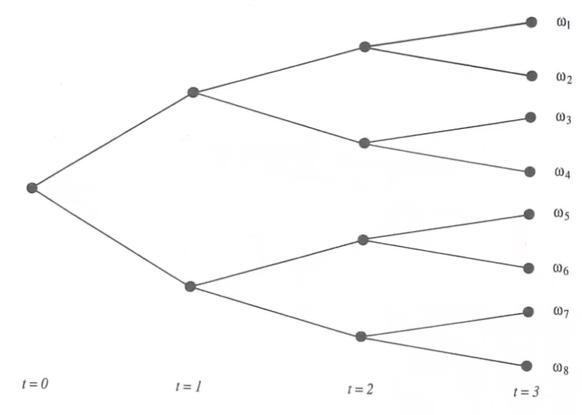
\includegraphics[width=.7\textwidth]{TreeOfInformationStructures.PNG}
    \caption{Tree diagram for the structure of information from \texttt{Example \ref{sec_stochastic_processes_in_discrete_time}.\ref{example_information_structures}.}}
    \label{fig_tree_diagram_of_information_structure}
  \end{figure}

  \begin{figure}[H]
    \centering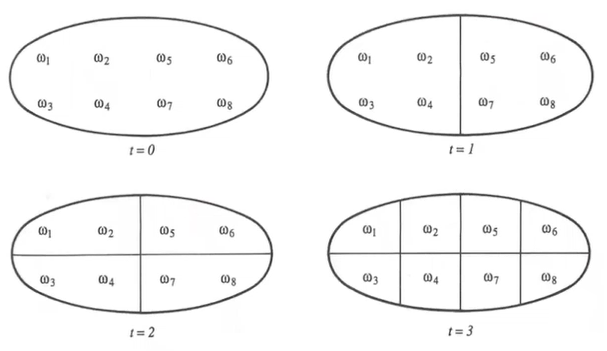
\includegraphics[width=.7\textwidth]{PicturesOfInformationStructures.PNG}
    \caption{A sequence of pictures demonstrating the structure of information \texttt{Example \ref{sec_stochastic_processes_in_discrete_time}.\ref{example_information_structures}.}}
    \label{fig_sequence_of_pictures_of_information_structure}
  \end{figure}

  \begin{example}{}
    Consider an arbitrary sequence $\{\hat{A}_t\}_{t\in[1,T]}$ and some time-point $s<T$. For each $\omega\in \hat{A}_s$ the sequence $\{A_t\}_{t\in[1,T]}$ with $A_T=\{\omega\}$ will coincide with $\{\hat{A}_t\}$ at least until time $t=s$.
    \par The collection of subsets $\{A_{s+1}\}$ that can follow $\hat{A}_s$ forms a partition of $\hat{A}_s$, that is, a collection of disjoint subsets whose union equals $\hat{A}_s$.
    \par In particular, taking $s=0$, we see that the collection $\{A_1\}$ of all possible time-period $t=1$ subsets forms a partition of $\Omega$. This partition is denoted $\mathcal{P}_1$.
    \par Moreover, the collection $\{A_2\}$ of all possible time-period $t=2$ subsets also forms a partition of $\Omega$, denoted $\mathcal{P}_2$.
    Consider \texttt{Example \ref{sec_stochastic_processes_in_discrete_time}.\ref{example_information_structures}} where $K=8$ and $T=3$, the partitions are
    \[\begin{array}{rcl}
      \mathcal{P}_0&=&\big\{\{\omega_1,\omega_2,\omega_3,\omega_4,\omega_5,\omega_6,\omega_7,\omega_8\}\big\}\\
      \mathcal{P}_1&=&\big\{\{\omega_1,\omega_2,\omega_3,\omega_4\},\{\omega_5,\omega_6,\omega_7,\omega_8\}\big\}\\
      \mathcal{P}_2&=&\big\{\{\omega_1,\omega_2\},\{\omega_3,\omega_4\},\{\omega_5,\omega_6\},\{\omega_7,\omega_8\}\big\}\\
      \mathcal{P}_3&=&\big\{\{\omega_1\},\{\omega_2\},\{\omega_3\},\{\omega_4\},\{\omega_5\},\{\omega_6\},\{\omega_7\},\{\omega_8\}\big\}\\
    \end{array}\]
  \end{example}

  \begin{remark}{Visualising Information Structure}
    There are two popular ways to visualise information structure
    \begin{enumerate}
      \item A \textit{Tree Diagram} where each node corresponds to an element $A_t$ of the time $t$ partition and where there is edge arc going from this node to each node corresponding to some $A_{t+1}\subseteq A_t$. (See \texttt{Figure \ref{fig_tree_diagram_of_information_structure}}).
      \item A \textit{Sequence of Pictures} of the same space. (See \texttt{Figure \ref{fig_sequence_of_pictures_of_information_structure}}).
    \end{enumerate}
  \end{remark}

  \begin{definition}{$\sigma$-Algebra $\mathcal{F}_t$}
    A collection $\mathcal{F}$ of subsets of $\Omega$ is called a \textit{$\sigma$-Algebra} on sample space $\Omega$ if
    \begin{enumerate}
      \item $\Omega\in\mathcal{F}$.
      \item $\forall\ F\in\mathcal{F},\ F^c\in\mathcal{F}$.
      \item $\forall\ F,G\in\mathcal{F},\ (F\cup G)\in\mathcal{F}$.
    \end{enumerate}
  \end{definition}

  \begin{proposition}{Generated $\sigma$-Algebra}
    For any partition $\mathcal{P}$ of $\Omega$ we can generate \textit{$\sigma$-Algebra} $\mathcal{F}$ by letting $\mathcal{F}$ be the collection of all unions of elements of $\mathcal{P}$ together with the complements of all such unions.
    \par Hence, the sub-models of the information structure can be organised as a sequence $\{\mathcal{F}_t\}_{t\in[1,T]}$ of \textit{$\sigma$-Algebras}.
  \end{proposition}

  \begin{definition}{Filtration $\mathcal{F}$}
    A \textit{Filtration} is a family of \textit{$\sigma$-Algebras} $\mathcal{F}:=\{\mathcal{F}_t:t=0,1,\dots,T\}$ where
    \begin{enumerate}
      \item $\mathcal{F}_0=\{\emptyset,\Omega\}$.
      \item $\mathcal{F}_T$ consists of all subsets of $\Omega$.
      \item $\mathcal{F}_n\subset\mathcal{F}_{n+1}$ for all $n<T$, by which we mean that each subset of $\mathcal{F}_n$ must be an element of $\mathcal{F}_{n+1}$.
    \end{enumerate}
  \end{definition}

  \begin{example}{$\sigma$-Algebra}
    Consider the context of \texttt{Example \ref{sec_stochastic_processes_in_discrete_time}.\ref{example_information_structures}}. The corresponding filtration is given by
    \[\begin{array}{rcl}
      \mathcal{F}_0&=&\big\{\emptyset,\Omega\big\}\\

      \mathcal{F}_1&=&\big\{\emptyset,\Omega,\{\omega_1,\omega_2,\omega_3,\omega_4\},\{\omega_5,\omega_6,\omega_7,\omega_8\}\big\}\\

      \mathcal{F}_2&=&\big\{\emptyset,\Omega,\{\omega_1,\omega_2\},\{\omega_3,\omega_4\},\{\omega_5,\omega_6\},\{\omega_7,\omega_8\},\{\omega_1,\omega_2,\omega_3,\omega_4\},\\
      &&\ \{\omega_5,\omega_6,\omega_7,\omega_8\},\{\omega_1,\omega_2,\omega_5,\omega_6\},\{\omega_1,\omega_2,\omega_7,\omega_8\},\{\omega_3,\omega_4,\omega_5,\omega_6\},\\
      &&\ \{\omega_3,\omega_4,\omega_7,\omega_8\},\{\omega_1,\omega_2,\omega_3,\omega_4,\omega_5,\omega_6\},\{\omega_1,\omega_2,\omega_3,\omega_4,\omega_7,\omega_8\},\\
      &&\ \{\omega_1,\omega_2,\omega_5,\omega_6,\omega_7,\omega_8\},\{\omega_3,\omega_4,\omega_5,\omega_6,\omega_7,\omega_8\}\big\}\\
    \end{array}\]
    and $\mathcal{F}_3$ contains all the subsets of $\Omega$ (ie $\mathcal{F}_3=2^\Omega$).
  \end{example}

\subsection{Stochastic Processes in Discrete Time}

  \begin{definition}{Stochastic Process $S$}
    A \textit{Stochastic Process} $S$ is a real-valued function $S(t)(\omega)$ of two variables, $t$ and $\omega$.
    \par For each fixed $\omega\in\Omega$ the function mapping $t\to S(t)(\omega)$ is called the \textit{Sample Path}.
    \par For each fixed $t\in[0,T]$ the function mapping $\omega\to S(t)(\omega)$ is a \textit{Random Variable}.
    \par NB - For simplicity, we assume $S(0)$ is constant.
  \end{definition}

  \begin{definition}{Measurable Function}
    A function $\omega\to W(\omega)$ is said to be \textit{Measurable} wrt the \textit{$\sigma$-Algebra} $\mathcal{F}$ if
    \begin{center}
      All $x\in\reals$ where $x\in W^{-1}(x)$ is an element of the \textit{$\sigma$-Algebra} $\mathcal{F}$.
    \end{center}
    where $W^{-1}(x):=\big\{\omega\in\Omega:W(\omega)=x\big\}$.\footnote{Equivalently, if we know which set of the \textit{$\sigma$-algebra} $\omega$ is in, then we know the value of $W(\omega)$.}
  \end{definition}

  \begin{example}{Measurable Function}
    Consider random variables $X,Y$ defined as
    \[\begin{array}{rcl}
      X(\omega)&=&\begin{cases}
        5&,\omega\in\{\omega_1,\omega_2,\omega_3,\omega_4\}\\
        7&,\omega\in\{\omega_5,\omega_6,\omega_7,\omega_8\}
      \end{cases}\\
      Y(\omega)&=&\begin{cases}
        8&,\omega\in\{\omega_1,\omega_3,\omega_5,\omega_7\}\\
        6&,\omega\in\{\omega_2,\omega_4,\omega_6,\omega_8\}
      \end{cases}
    \end{array}\]
    Then, by the notation of \texttt{Example \ref{sec_stochastic_processes_in_discrete_time}.\ref{example_information_structures}}, we have that
    \begin{itemize}
      \item $X$ is \textit{Measurable} wrt $\mathcal{F}_1,\mathcal{F}_2,\mathcal{F}_3$ as $\big\{\{\omega_1,\omega_2,\omega_3,\omega_4\},\{\omega_5,\omega_6,\omega_7,\omega_8\},\emptyset\big\}\subset\mathcal{F}_1$.
      \item $Y$ is \underline{not} \textit{Measurable} wrt $\mathcal{F}_1,\mathcal{F}_2$, but is measurable wrt $\mathcal{F}_3$, as $\{\omega_1,\omega_3,\omega_5,\omega_7\}\not\in\mathcal{F}_1$.
    \end{itemize}
  \end{example}

  \begin{remark}{Measurable}
    If a function $X$ is \textit{Measurable} wrt $\mathcal{F}_t$ then it will be \textit{Measurable} wrt $\mathcal{F}_{t+1}$, as $\mathcal{F}_t\subseteq\mathcal{F}_{t+1}$.
  \end{remark}

  \begin{definition}{Adapted}
    A \textit{Stochastic Process} $S=\{S(t):t=0,1,\dots,T\}$ is said to be \textit{Adapted} to the \textit{Filtration} $\mathcal{F}=\{\mathcal{F}_t:t=0,1,\dots,T\}$ if for every $t=0,\dots,T$ the random variable $S(t)$ is \textit{Measurable} wrt $\mathcal{F}_t$.
  \end{definition}

  \begin{remark}{Adapted Filtrations in Practice}
    In practice we often define the \textit{Stochastic Process} $S$ first and use the so-called ``\textit{Natural Filtration}'', defined as
    \begin{enumerate}
      \item For each $t=0,1,\dots,T$ let $\mathcal{P}_t$ be the partition of $\Omega$ st the \textit{Stochastic Process} $\{S(0),\dots,S(t)\}$ takes the same value for each $\omega\in A$, for each subset $A\in\mathcal{P}_t$.
      \item Let $\mathcal{F}_t$ be the \textit{$\sigma$-Algebra} generated by $\mathcal{P}_t$.
      \item Then $\mathcal{F}:=\{\mathcal{F}_t:t=0,1,\dots,T\}$ is called the filtration \textit{Generated} by the \textit{Stochastic Process} $S$.
    \end{enumerate}
  \end{remark}

  \begin{example}{}
    Consider the setting it \texttt{Example \ref{sec_stochastic_processes_in_discrete_time}.\ref{example_information_structures}} and let $S(t)$ be the upwards movements in the value of the asset by time $t$. Then $S(t)$ generates the \textit{Filtration} above.
    \par This can be summarised in the table
    \begin{center}
      \begin{tabular}{c|cccc}
        $\omega_k$&$t=0$&$t=1$&$t=2$&$t=3$\\\hline
        $\omega_1$&$S(t)=0$&$S(t)=1$&$S(t)=2$&$S(t)=3$\\
        $\omega_2$&$S(t)=0$&$S(t)=1$&$S(t)=2$&$S(t)=2$\\
        $\omega_3$&$S(t)=0$&$S(t)=1$&$S(t)=1$&$S(t)=2$\\
        $\omega_4$&$S(t)=0$&$S(t)=1$&$S(t)=1$&$S(t)=1$\\
        $\omega_5$&$S(t)=0$&$S(t)=0$&$S(t)=1$&$S(t)=2$\\
        $\omega_6$&$S(t)=0$&$S(t)=0$&$S(t)=1$&$S(t)=1$\\
        $\omega_7$&$S(t)=0$&$S(t)=0$&$S(t)=0$&$S(t)=1$\\
        $\omega_8$&$S(t)=0$&$S(t)=0$&$S(t)=0$&$S(t)=0$
      \end{tabular}
    \end{center}
  \end{example}

  \begin{definition}{Random Walk}
    Let $X_t:=X_0+Y_1+\dots+Y_t$ where $Y_1,\dots,Y_t$ are iid random variables with finite variance $\sigma^2$ and mean $mean$. Then $\{X_t:t\geq0\}$ is a \textit{Random Walk}.
    \par We say that $\{X_t:t\geq0\}$ is a \textit{Simple Random Walk} if $Y_i$ takes only the values 1 with probability $p$ and -1 with probability $1-p$.
  \end{definition}

  \begin{proposition}{Distribution of Simple Random Walk Values}
    A \textit{Simple Random Walk} takes values $y$ at time-point $t$ iff exactly $\frac{t+y}2$ of $Y_1,\dots,Y_t$ are equal to 1, and the remaining $\frac{t-y}2$ equal -1.
    \[ \forall\ t\geq0,y\in\{-t,-t+2,\dots,t-2,t\},\quad\prob(X_t=y)={t\choose {\frac{t+y}2}}p^{(t+y)/2}(1-p)^{(t-y)/2} \]
  \end{proposition}

\subsection{Conditional Expectations}

\subsection{Martingales}

\subsection{Stopping Times}

\section{Multi-Period Models} \label{sec_multi_period_models}

\subsection{Trading Strategies}

\subsection{Arbitrage in Multi-Period Model and Martingale Measures}

\subsection{Valuation of Contingent Claims}

\subsection{American Claims}

\subsection{The Cox-Ross Rubinstein Model}

\subsection{The Cox-Ross Rubinstein Model and the Black-Scholes Formula}

\section{Stochastic Processes in Continuous Time} \label{sec_stochastic_processes_in_continuous_time}

\subsection{The Brownian Motion}

\subsection{Stochastic Integration}

\subsection{It\^o's Lemma}

\section{Financial Market Models in Continuous Time} \label{sec_financial_market_models_in_continuous_time}

\subsection{The Financial Market Model in Continuous Time}

\subsection{Trading Strategies}

\subsection{Arbitrage in the Continuous Time Model}

\subsection{The Black-Scholes Model}

\subsection{Equivalent Martingale Measures in the Black-Scholes Model}

\subsection{Pricing in the Black-Scholes Model}

\subsection{Replicating Strategies and the Black-Scholes-Merton Equation}

\reference
\section{Notation}

  \begin{notation}{General Mathematical Notation}
    \begin{tabular}{c|c}
      Notation&Description\\\hline
      $\{x\}_+$&Only the positive part of $x$ (i.e. $\max\{0,x\}$).
    \end{tabular}
  \end{notation}

\end{document}
